\renewcommand{\sectionbreak}{}
\section{Problématique et objectif}

En culture hors-sol (\textbf{figure \ref{fig1}}), il faut constamment déplacer
les pots pour profiter de la lumière, pour regrouper les cultures,
isoler celles qui posent problème, ... Ce travail est pénible physiquement et les pépiniéristes peinent à trouver de la main d'œuvre
pour réaliser ces tâches quotidiennes difficiles.

\begin{figure}[!htb]
\begin{minipage}{0.5\textwidth}
\begin{center}
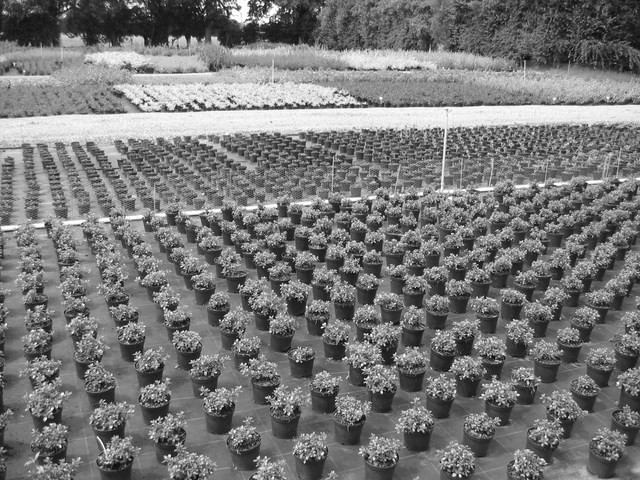
\includegraphics[width=0.95\textwidth]{images/image1.jpg}
\caption{Exemple de culture hors-sol  \label{fig1}}
\end{center}
\end{minipage}
\begin{minipage}{0.5\textwidth}
\begin{center}
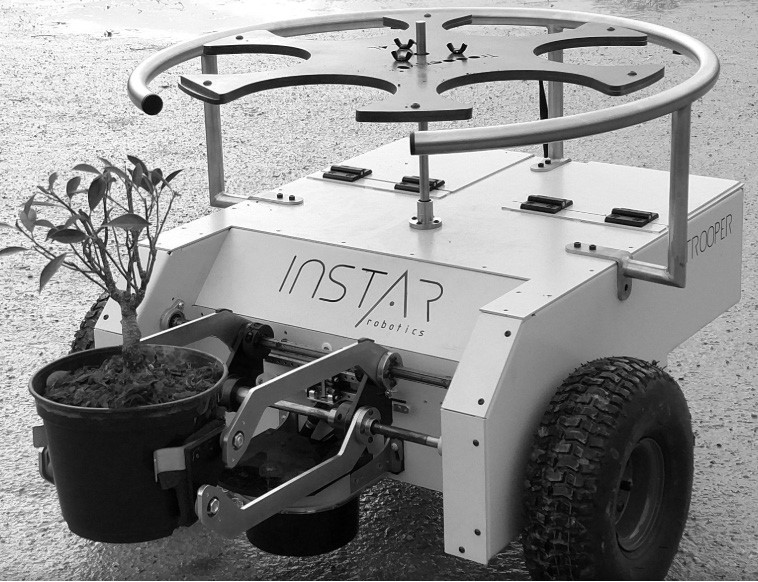
\includegraphics[width=0.95\textwidth]{images/image2.jpg}
\caption{Robot TROOPER de la société \textbf{INSTAR ROBOTICS} \label{fig2}}
\end{center}
\end{minipage}
\end{figure}


La Startup INSTAR ROBOTICS, spécialisée dans le développement de robots
d'assistance, a conçu le robot TROOPER qui permet de répondre à ce
besoin (\textbf{figure \ref{fig2}}).

L'objectif du travail proposé dans cette épreuve est de justifier les
solutions techniques retenues par la société INSTAR ROBOTICS dans le but
de respecter le cahier des charges élaboré en partenariat avec des
pépiniéristes.

\section{Cahier des charges}\label{partie-ii---cahier-des-charges}


Les spécifications que doit respecter le robot sont directement liées
aux contraintes imposées par la culture hors-sol.

Une des contraintes majeures est la vitesse à laquelle le robot doit se
déplacer et réaliser les opérations de prise/dépose de pots afin d'être
si possible aussi rapide qu'une personne.

Un exemple de tâche à réaliser consiste à déplacer 4 rangées de 6 pots
d'une zone à une autre. Le robot doit prendre les 6 pots de la rangée 1
de la zone 1, puis les déplacer dans la rangée 1 de la zone 2, de même
pour les autres rangées.

On note \emph{T\textsubscript{p}} le temps de prise d'une rangée de 6
pots, égal au temps de dépose (ce temps inclut toutes les manœuvres et
est estimé à 30 s). On suppose que le robot se déplace à la vitesse
constante \emph{V} en ligne droite sur une distance \emph{L} = 10m
séparant les rangées de chaque zone (\textbf{figure \ref{fig3}}). La distance
entre deux rangées d'une zone est notée $l = 50cm$.


\begin{figure}[!htb]
\begin{center}
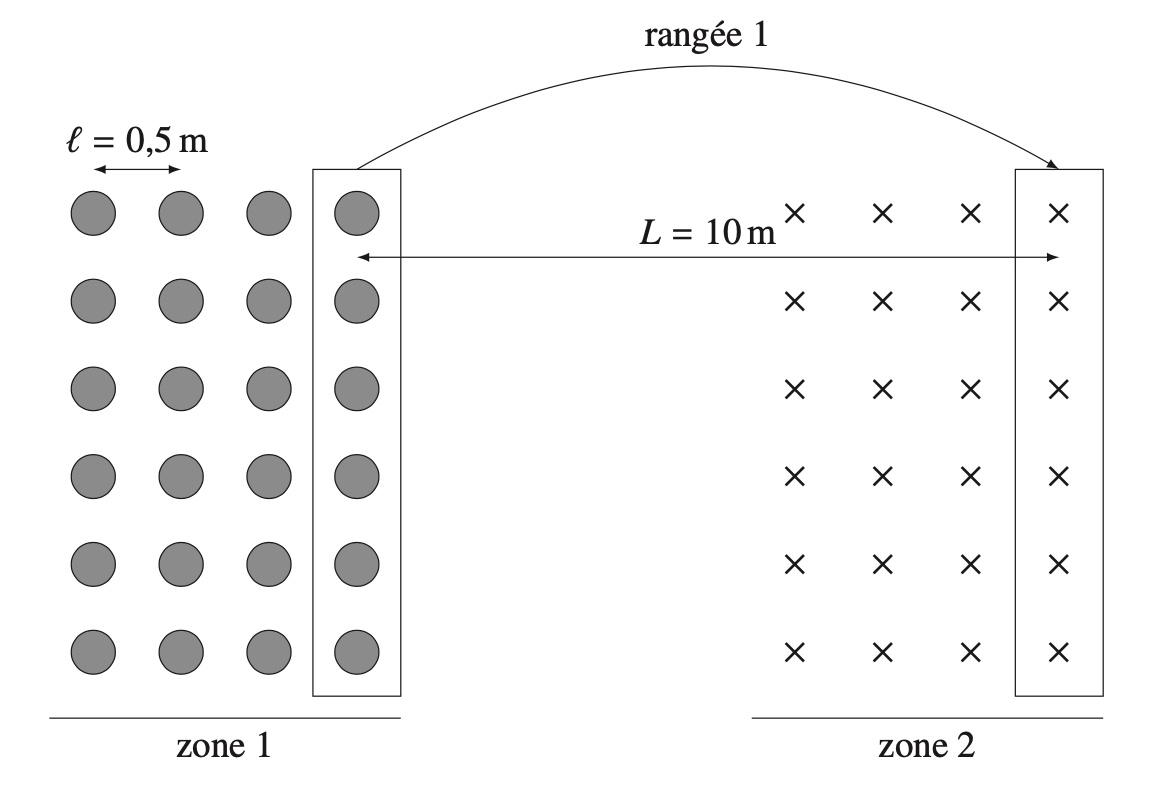
\includegraphics[width=0.8\textwidth]{images/fig3.jpg}
\caption{Tâche à effectuer par le robot  \label{fig3}}
\end{center}
\end{figure}


Un employé qui utilise un chariot à pousser (pour déplacer 6 pots à
chaque fois) met un temps total \emph{T\textsubscript{m} pour} réaliser
cette tâche de repositionnement de 4 rangées de pots.

\question{Déterminer la vitesse \emph{V}, supposée constante, à
laquelle doit se déplacer le robot en ligne droite pour réaliser la
tâche au maximum en \emph{T\textsubscript{m }}secondes en fonction de
\emph{L}, $l$, \emph{T\textsubscript{m }}et
\emph{T\textsubscript{p}}. Faire l'application numérique pour une durée
\emph{T\textsubscript{m }}de 320 secondes.}


Les autres éléments du cahier des charges pourraient être justifiés de
la même manière. Le diagramme des exigences de la \textbf{figure \ref{fig4}}
liste les éléments principaux utiles pour le dimensionnement du robot.

Le robot est constitué de plusieurs chaînes d'énergie et d'information.
Nous analyserons dans un premier temps les chaînes d'énergie et
d'information relatives au déplacement du robot, puis, dans un second
temps, celles relatives à la prise et dépose des pots.

Pour se déplacer, le robot utilise deux roues motorisées indépendantes à
l'avant et deux roues folles à l'arrière. Le robot embarque une batterie
pouvant délivrer jusqu'à 100 Volts. Une carte de commande dédiée à
chaque moteur utilise l'information d'un codeur incrémental monté sur
chaque axe moteur pour donner des ordres au hacheur pilotant ce même
moteur. Un réducteur permet d'adapter la vitesse de rotation du moteur
pour la transmettre à la roue. Pour permettre au robot de se diriger
correctement, un dispositif LIDAR (Laser Imaging Detection And Ranging :
émetteur/récepteur infrarouge) fournit des informations sur
l'environnement à un micro-ordinateur qui se charge d'envoyer des
consignes aux cartes de commande des moteurs. L'utilisateur peut
communiquer avec le robot à l'aide d'une tablette en Bluetooth.

 

\question{À l'aide des informations ci-dessus, compléter les chaînes
d'énergie et d'information pour le déplacement du robot.}


\begin{figure}[!htb]
\begin{center}

\includegraphics[width=0.95\textwidth]{images/image3.png}
\caption{Diagramme des exigences du robot Trooper  \label{fig4}}
\end{center}
\end{figure}


\section{Déplacement du robot}

Nous allons montrer tout d'abord la nécessité d'asservir en vitesse les
moteurs pour assurer un déplacement correct du robot.

\subsection{Nécessité d'un asservissement en vitesse}

Chaque roue motorisée du robot a pour rayon $r = \SI{15}{cm}$ et le
rapport de réduction du réducteur associé à chaque moteur vaut
$k_r= 1/40$. Ainsi la vitesse de déplacement du robot est donné par  : 

\begin{align*}
V=k_r\cdot r\cdot \omega_m
\end{align*}

avec $\omega_m$, la vitesse de rotation à la sortie du moteur (en rad/s) et $V$ la vitesse de déplacement du robot en $m/s$.

Les caractéristiques d'un moteur sont :

\begin{itemize}
\item $J_m = \SI{3,4 1e-3}{kg \cdot m^2}$ moment
  d'inertie de l'ensemble motoréducteur ramené sur l'arbre moteur,
\item $k_m = \SI{0,2}{N.m.A^{-1}}$ constante de
  couple (égale à la constante de vitesse)
\item $R_m= \SI{1}{\Omega}$ résistance interne du moteur
\item vitesse maximale du moteur égale à $\SI{3000}{tr.min^{-1}}$.
\end{itemize}

\question{A l'aide du diagramme des exigences de la figure \ref{fig4}, donner l'identifiant de l'exigence permettant de vérifier le critère de vitesse maximale}



\question{Vérifier que les éléments choisis permettent de respecter
le critère de vitesse maximale défini dans le diagramme des exigences.}

\begin{minipage}{0.65\textwidth}
On souhaite que le robot se déplace selon une loi trapèze de vitesse
avec $V_{max}$ la vitesse maximale du robot (du
diagramme des exigences) pour parcourir une $D=10m$. On
donne le temps total $T=10s$ et on cherche la durée
d'accélération égale à la durée de décélération $\delta t$. Pour la
question suivante, on suppose, de manière simplifiée, que le robot suit
parfaitement cette consigne.
\end{minipage}
\begin{minipage}{0.35\textwidth}
\begin{center}
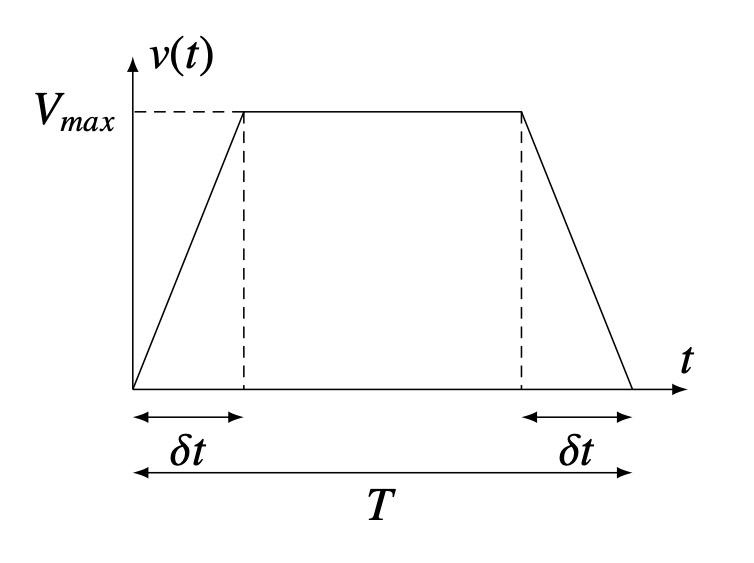
\includegraphics[width=0.95\textwidth]{images/trapeze}
\end{center}
\end{minipage}



\question{Déterminer l'expression du temps $\delta t$ pour respecter
le déplacement souhaité en fonction de $D$, $T$ et
$\V_{max}$. Faire l'application numérique.}


On suppose que les deux moteurs sont identiques. Les équations qui
caractérisent le comportement en ligne droite du robot sont les
suivantes :

\begin{itemize}
\item
  \[u_{m}\left( t \right) = R_{m}.i_{m}\left( t \right) + k_{m}.\omega_{m}\left( t \right)\]
  (1)
\item
  \[{2C}_{m}\left( t \right) - C_{r}\left( t \right) = J_m.\frac{d\omega_{m}\left( t \right)}{\text{dt}}\]
  (2)
\item
  \[C_{m}\left( t \right) = k_{m}.i_{m}\left( t \right)\] (3)
\item
  \[v\left( t \right) = k_{t}.\omega_{m}\left( t \right)\] (4)
\end{itemize}

où \(\omega_{m}\left( t \right)\) est la vitesse angulaire d'un moteur,
\(u_{m}\left( t \right)\) la tension de commande d'un moteur,
\(i_{m}\left( t \right)\) le courant traversant chaque moteur et
\(C_{m}\left( t \right)\) le couple exercé par un moteur.

\textbf{\emph{C\textsubscript{r}}(\emph{t}) est un couple résistant global
supposé nul} dans un premier temps pour les deux questions suivantes.
\emph{J} est le moment d'inertie équivalent de l'ensemble en mouvement
ramené sur un arbre moteur.

 \(v\left( t \right)\) est la vitesse du
robot en ligne droite par rapport au sol.


\question{Déterminer l'équation différentielle vérifiée par
\(v\left( t \right)\) avec \(u_{m}\left( t \right)\) comme entrée. On montrera qu'elle pourra se mettre sous la forme : $A\dfrac{d v(t)}{dt}+B\cdot v(t)=u_m(t)$ et on identifiera A et B en fonction des constantes du problèmes.}

On suppose que \emph{v}(0) = 0.

\question{Vérifier que \(v\left( t \right) = \alpha_{0}(t - \tau_{m} + \tau_{m}e^{- t/\tau_{m}})\)
est solution de l'équation différentielle pour une consigne de tension
\(u_{m}\left( t \right) = \frac{u_{0}}{\delta t}t\) pour $t \geq 0$.}


\question{On donnera l'expression de \(\alpha_{0}\) et \(\tau_{m}\) en fonction de
\(u_{0}\), \(\delta t\) et des constantes intervenant dans les
équations du moteur.}


La \textbf{figure \ref{fig5}} montre la réponse du robot à une tension de
commande en trapèze. La courbe de vitesse simulée est tracée ainsi que
la courbe de vitesse de consigne fournie (qui correspond ici directement à la tension $u_m(t)$.

On donne dans le document réponse une partie du programme codé en python3 qui a permis de résoudre l'équation différentielle et de tracer cette courbe.
La vitesse de consigne en pointillé correspond à $u_m(t)$ et est défini par un trapèze parfait sur la figure \ref{fig5}.

\question{Compléter la partie permettant de définir les fonctions \texttt{F(y,t}) et \texttt{u\_m(t)} qui permettent d'obtenir le la liste \texttt{vt} par la méthode d'Euler.}

La deuxième courbe de la \textbf{figure \ref{fig5}} est obtenue par intégration numérique de la fonction \texttt{vt} et correspond à la position du robot au cours du temps. 

\question{Proposer une méthode d'intégration numérique permettant d'obtenir cette courbe à partie de la liste \texttt{vt}. Écrire sous la forme d'une fonction codée en python3 les instructions correspondantes.}


\begin{figure}[!htb]
\begin{center}
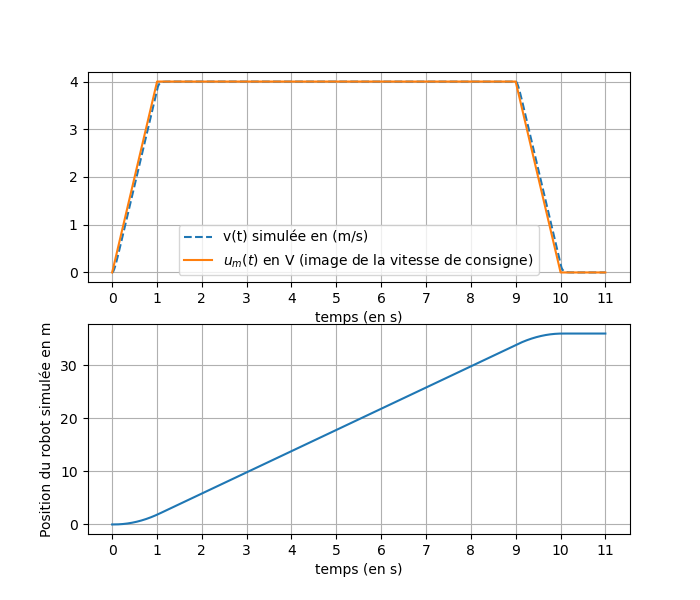
\includegraphics[width=0.8\textwidth]{images/figure5.png}
\caption{Simulation du déplacement du robot en réponse à une consigne en trapèze  \label{fig5}}
\end{center}
\end{figure}

\question{En s'aidant de l'expression de la vitesse donnée
précédemment, estimer la valeur de \(\tau_{m}\) à partir de la courbe de
vitesse réelle. Faire apparaître le tracé sur la figure du
\textbf{Document Réponse}.}


Au regard des simulations effectuées, on constate qu'on peut confondre
la vitesse de consigne avec la vitesse simulée et ainsi travailler
directement avec le profil de vitesse de consigne pour des études
cinématiques.

Le robot évolue sur un terrain souvent boueux et accidenté, ce qui
engendre des perturbations sur les roues, le robot ne se déplace alors
plus à la vitesse souhaitée. De plus, pour des courants trop faibles,
les roues ne tournent pas à cause des frottements. La vitesse de
déplacement du robot est donc asservie à une vitesse de consigne notée
\(v_{c}(t)\).


Un adaptateur de gain $K_{a}$ convertit la consigne \(v_{c}(t)\) ($m\cdot s^{-1}$) en une valeur numérique notée $n_c(t)$.
Cette valeur numérique est comparée à l'image $n_m(t)$ de la vitesse de rotation des moteurs \(\omega_{m}\left( t \right)\)
déterminée à l'aide d'un codeur incrémental de gain $K_c$. Celui-ci délivre 628 informations (ou inc) par tour de moteur.



L'écart $\varepsilon(t)$ ainsi formé est adapté par un ensemble correcteur
amplificateur dont la fonction de transfert sera notée $C(p)$ pour fournir la tension d'alimentation
\(u_{m}\left( t \right)\) aux moteurs.

La vitesse de rotation des moteurs \(\omega_{m}\left( t \right)\) est
adaptée par l'ensemble réducteur-roue de gain $k_t$ pour obtenir la vitesse \emph{v}(\emph{t}) de déplacement du robot.

Des perturbations sur les moteurs sont prises en compte sous la forme
d'un couple résistant noté $C_r(t)$.


\question{À partir des équations (1), (2) et (3), déterminer
la relation \(\Omega_{m}\left( p \right) = H_{m}\left( p \right).U_{m}\left( p \right) + H_{r}\left( p \right).C_{r}\left( p \right)\)
où l'on précisera l'expression de \(H_{m}\left( p \right)\) et
\(H_{r}\left( p \right)\) sous forme canonique.}

\question{Compléter le schéma-bloc de l'asservissement de vitesse
linéaire du robot en utilisant les indications précédentes.}

\question{Préciser la
valeur numérique de $K_c$ en \emph{inc}/\emph{rad}.
Donner l'expression de $K_a$ permettant d'assurer un
asservissement correct.}


On choisit de prendre un correcteur proportionnel intégral de la forme
\(C\left( p \right) = K_{p}\frac{1 + \tau_{i}p}{\tau_{i}p}\)


On prend pour valeur de \(\tau_{i}\) la valeur de la constante de temps
du moteur : \(\tau_{i} = \tau_{m}=0,1s\).

\question{Tracer sur le document réponse le diagramme de Bode asymptotique du correcteur $C(p)$ avec $K_p=1$. Veillez à bien justifier votre réponse.}

Compte tenu de la valeur choisie pour \emph{K\textsubscript{a}}, le
schéma-bloc de l'asservissement de vitesse peut être mis sous forme de
schéma-bloc à retour unitaire dont la Fonction de Transfert en Boucle
Ouverte est :

\[\text{FTBO}\left( p \right) = C(p) \frac{K_{m}K_{c}}{{1 + \tau}_{m}p}\]

avec $K_{m}K_{c} = 500 inc\cdot s^{-1}\cdot V^{-1}$ et $\tau_{m} = 0,1s$.

\question{Calculer la fonction de transfert en boucle fermée du système et la mettre sous forme canonique.}

\question{Déterminer la valeur de $K_p$ pour que
le temps de réponse à $5 \%$ en boucle fermée soit égal à $0,3s$.}

\question{Tracer le diagramme de Bode de $FTBO(p)$ avec la valeur de $K_p$ trouvée précédemment. Conclure sur la stabilité du système et donnant les marges de stabilité.}


\question{En considérant toujours un retour unitaire, donner l'expression de $\varepsilon(p)=V_c(p)-V(p)$ en fonction de $V_c(p)$ et des constantes de la $FTBO$.}

\begin{itemize}
\item On rappelle que l'erreur statique est la limite en $+\infty$ de $\varepsilon(t)$ avec $v_c(t)$ un échelon d'amplitude $v_{c1}$.
\item On rappelle que l'erreur statique est la limite en $+\infty$ de $\varepsilon(t)$ avec $v_c(t)$ une rampe d'amplitude $v_{c2}$.
\end{itemize}


\question{Déterminer alors la précision du système dans ces deux cas.}

La \textbf{figure 6} représente la réponse du robot pour une consigne en
trapèze en utilisant un correcteur bien réglé et en prenant en compte
des perturbations de type frottement sec. Pour prendre en compte le
couple \emph{C\textsubscript{r }}dans la simulation, un bloc
non-linéaire a été introduit dans le schéma-bloc pour aboutir à cette
réponse.


\begin{figure}[!htb]
\begin{center}

\includegraphics[width=0.9\textwidth]{images/image7.png}
\caption{Simulation de la vitesse du robot asservi en réponse à une consigne en trapèze  \label{fig6}}
\end{center}
\end{figure}


\question{Entourer sur la courbe la zone qui montre que la
perturbation a été prise en compte. Préciser quelle non-linéarité (à
choisir parmi saturation, seuil, hystérésis) a été retenue. Conclure sur
la pertinence de l'asservissement de vitesse mis en place vis-à-vis des
performances attendues.}

\section{Comportement en pente}\label{iii.2---comportement-en-pente}

La motorisation retenue permet de déplacer le robot sur sol horizontal
même en présence d'une perturbation de type frottement sec. Il faut
cependant vérifier qu'elle permet également au robot de gravir des
pentes.

\question{Donner le(s) exigence(s) sur le diagramme de la figure \ref{fig4} qui permettent de vérifier les performances dans ce cas. Donner alors les grandeurs quantifiable.}


On se place dans le cas où le robot supporte 6 pots de masse $m=\SI{10}{kg}$ chacun. On note $M = \SI{60}{kg}$ la masse du robot. On associe au sol le repère
\((O,\ \overrightarrow{x},\ \overrightarrow{y_{0}},\ \overrightarrow{z_{0}})\)
incliné d'un angle \(\alpha = \left( \ \overrightarrow{y},\ \overrightarrow{y_{0}} \right) = \left( \ \overrightarrow{z},\ \overrightarrow{z_{0}} \right)\)
constant par rapport à l'horizontale.

Le robot se déplace en ligne droite selon
\((O,\ \overrightarrow{y_{0}})\) à la vitesse \emph{v}(\emph{t}), en
phase de montée. On note \emph{C\textsubscript{m}}(\emph{t}) le couple
appliqué par chaque moteur pour faire avancer le robot. Les liaisons
sont toutes supposées parfaites énergétiquement et le robot roule sans
glisser sur le sol (\textbf{figure \ref{fig7}}).



On rappelle que\(\text{\ v}\left( t \right) = k_{t}.\omega_{m}\left( t \right)\). On
négligera l'inertie des réducteurs et des roues.

On peut montrer, en appliquant le théorème de l'énergie cinétique
au robot en mouvement, que l'équation qui décrit le mouvement du robot
en pente est la suivante :

\begin{align*}
M_{\text{eq}}\frac{dv(t)}{\text{dt}} = \frac{1}{r_{\text{eq}}}C_{m}\left( t \right) - F_{r,eq}
\end{align*}

avec : 

\begin{itemize}
\item $M_{\text{eq}}=\SI{120}{kg}$,
\item $r_{eq} =\SI{2e-3}{m}$,
\item $F_{r,eq}= \SI{200}{N}$.
\end{itemize}
%%%%

\begin{figure}[!htb]
\begin{center}
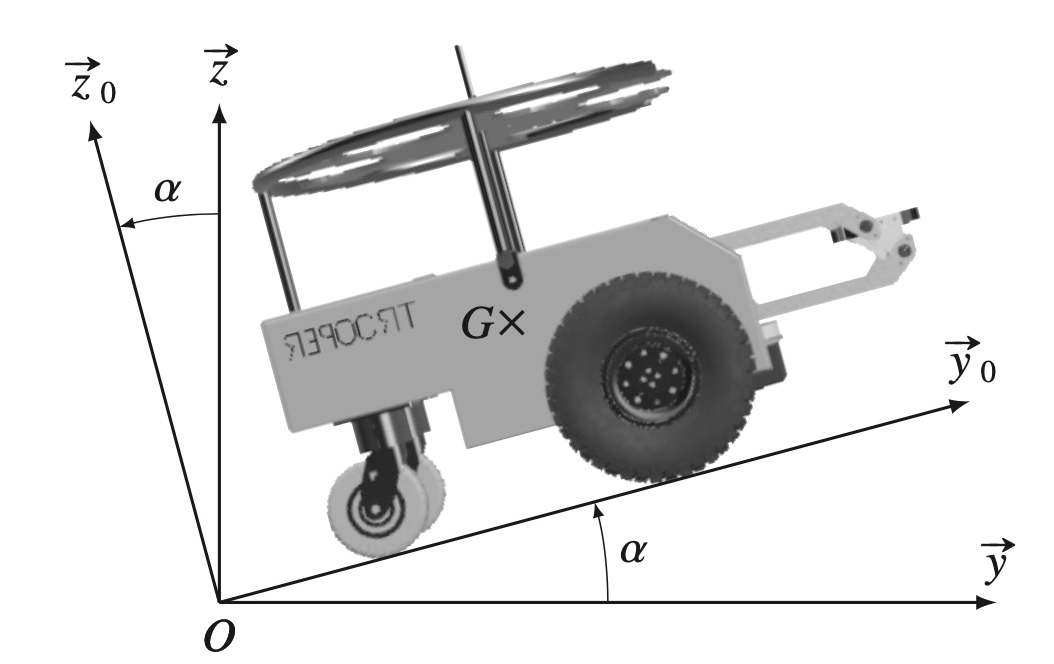
\includegraphics[width=0.6\textwidth]{images/parametrage_pente}
\caption{Paramétrage pour l’étude en pente du robot (représenté sans les pots) \label{fig7}}
\end{center}
\end{figure}


\begin{minipage}{0.35\textwidth}
On considère à nouveau la loi de pilotage définie précédemment sous
forme de trapèze avec $V_{max}=1,1m\cdot s^-1$, $\delta t=1s$ et $T=10s$.
\end{minipage}
\begin{minipage}{0.65\textwidth}
\begin{center}
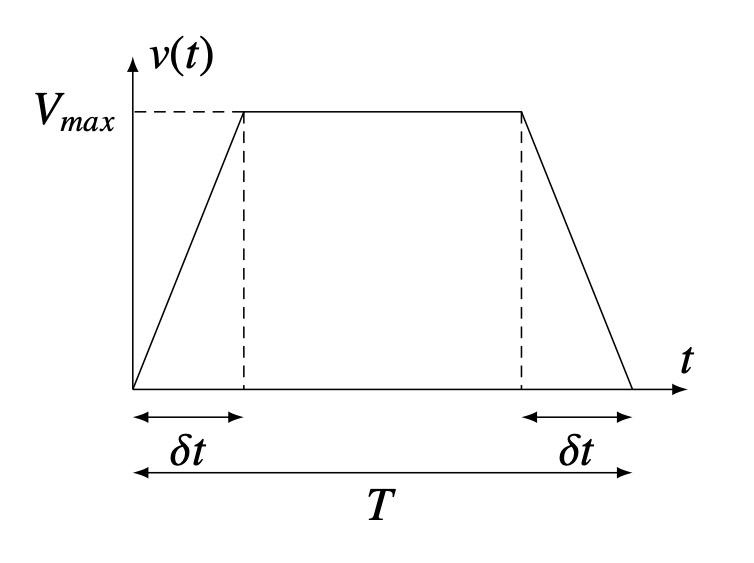
\includegraphics[width=0.95\textwidth]{images/trapeze}
\end{center}
\end{minipage}

\question{Tracer l'évolution de \emph{C\textsubscript{m}}(\emph{t})
au cours du temps compte tenu de l'évolution souhaitée de
\emph{v}(\emph{t}). Préciser les valeurs caractéristiques sous forme
littérale, puis numérique.}




\question{À l'aide des équations du moteur, déterminer le couple
maximal développé par un moteur lorsqu'il est alimenté sous 100 V.
Vérifier alors que la motorisation est adaptée à une montée en pente du
robot.}


%\section{Comportement en pente}\label{iii.2---comportement-en-pente}}
%
%La motorisation retenue permet de déplacer le robot sur sol horizontal
%même en présence d'une perturbation de type frottement sec. Il faut
%cependant vérifier qu'elle permet également au robot de gravir des
%pentes comme indiqué dans le diagramme des exigences (Id 1.2.1), ce qui
%correspond à une perturbation supplémentaire.
%
%%On se place dans le cas où le robot supporte 6 pots de masse $m=\SI{10}{kg}$ chacun. On note $M = \SI{60}{kg}$ la masse du robot. On associe au
%%sol le repère
%\((O,\ \overrightarrow{x},\ \overrightarrow{y_{0}},\ \overrightarrow{z_{0}})\)
%incliné d'un angle
%\(\alpha = \left( \ \overrightarrow{y},\ \overrightarrow{y_{0}} \right) = \left( \ \overrightarrow{z},\ \overrightarrow{z_{0}} \right)\)
%constant par rapport à l'horizontale.
%
%Le robot se déplace en ligne droite selon
%\((O,\ \overrightarrow{y_{0}})\) à la vitesse \emph{v}(\emph{t}), en
%phase de montée. On note \emph{C\textsubscript{m}}(\emph{t}) le couple
%appliqué par chaque moteur pour faire avancer le robot. Les liaisons
%sont toutes supposées parfaites énergétiquement et le robot roule sans
%glisser sur le sol (\textbf{figure 7}).
%
%%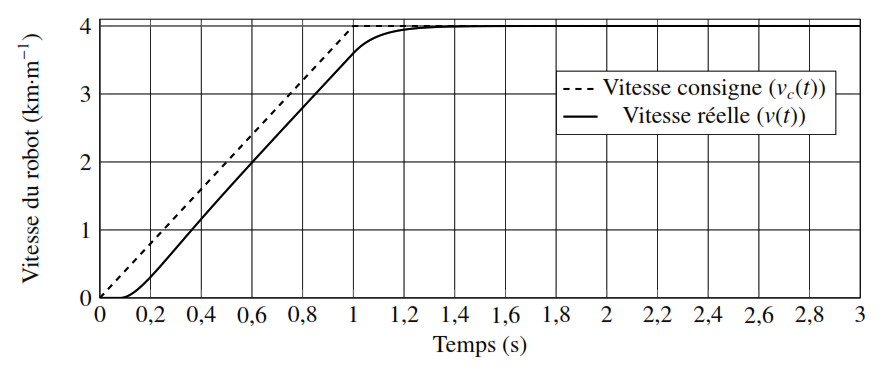
\includegraphics[width=5.36198in,height=2.58436in]{images/image5.png}
%
%On rappelle
%que\(\text{\ v}\left( t \right) = k_{t}.\omega_{m}\left( t \right)\). On
%négligera l'inertie des réducteurs et des roues.
%
%On peut montrer, en appliquant le théorème de l'énergie cinétique
%au robot en mouvement, que l'équation qui décrit le mouvement du robot
%en pente est la suivante :

%\begin{align*}
%M_{\text{eq}}\frac{dv(t)}{\text{dt}} = \frac{1}{r_{\text{eq}}}C_{m}\left( t \right) - F_{r,eq}
%\end{align*}
%
%avec : 
%
%\begin{itemize}
%\item $M_{\text{eq}}=\SI{120}{kg}$,
%\item $r_{eq} =\SI{2\cdot 1e-3}{m}$,
%\item $F_{r,eq}= \SI{200}{N}$.
%\end{itemize}


%On considère à nouveau la loi de pilotage définie précédemment sous
%forme de trapèze avec \emph{V\textsubscript{max }}=
%1,1m·s−\textsuperscript{1}, δ\emph{t} = 1s et \emph{T} = 10s.
%
%\textbf{Q13.} Tracer l'évolution de \emph{C\textsubscript{m}}(\emph{t})
%au cours du temps compte tenu de l'évolution souhaitée de
%\emph{v}(\emph{t}). Préciser les valeurs caractéristiques sous forme
%littérale, puis numérique.
%
%\textbf{Q14.} À l'aide des équations du moteur, déterminer le couple
%maximal développé par un moteur lorsqu'il est alimenté sous 100 V.
%Vérifier alors que la motorisation est adaptée à une montée en pente du
%robot.


\subsection{Annexes}


Pour rappel : $u(t)$ est la fonction échelon unitaire.
\renewcommand\arraystretch{1.3}
\begin{center}
\begin{tabular}{|c|c||c|c|}
	\hline
	$f(t)$			&		$\displaystyle F(p)=\L\left[f(t)\right]$		&	$f(t)$				&	$F(p)=\L\left[f(t)\right]$			\\[0.3cm]
	\hline\hline
	$u(t)$			&		$\displaystyle \frac 1p$				&	$\sin(\omega t)\;u(t)$		&	$\displaystyle \frac{\omega}{p^2+\omega^2}$	\\[0.3cm]
	\hline
	$K\;u(t)$		&		$\displaystyle \frac{K}{p}$				&	$\cos(\omega t)\;u(t)$		&	$\displaystyle \frac{p}{p^2+\omega^2}$		\\[0.3cm]
	\hline
	$K\;t\;u(t)$		&		$\displaystyle \frac K{p^2}$				&	$\sinh(\omega t)\;u(t)$		&	$\displaystyle \frac \omega{p^2-\omega^2}$	\\[0.3cm]
	\hline
	$e^{-at}u(t)$		&		$\displaystyle \frac{1}{p+a}$				&	$\cosh(\omega t)\;u(t)$		&	$\displaystyle \frac{p}{p^2-\omega^2}$		\\[0.3cm]
	\hline
	$t^nu(t)$		&		$\displaystyle \frac{n!}{p^{n+1}}$			&	$e^{-at}\sin(\omega t)u(t)$	&	$\displaystyle \frac \omega{(p+a)^2+\omega^2}$	\\[0.3cm]
	\hline
	$e^{at} t^n u(t)$	&		$\displaystyle \frac{n!}{(p-a)^{n+1}}$			&	$e^{-at}\cos(\omega t) u(t)$	&	$\displaystyle \frac{p+a}{(p+a)^2+\omega^2}$	\\[0.3cm]
	\hline
	$\delta(t)$		&		$1$							&	$K\;\delta(t)$			&	$K$						\\[0.3cm]
	\hline
\end{tabular}
\end{center}
